\documentclass[sigconf]{acmart}
% =============================================================================
% Template setup — participants normally do not edit this file.
% Author content belongs in main.tex; citations belong in main.bib.
% \documentclass lives in main.tex so Overleaf does not treat this file as root.
% =============================================================================

% --- Competition / non-ACM-submission friendly rights metadata -------------
\setcopyright{none}
\settopmatter{printacmref=false}
\acmConference[Kaggle Competition]{Filament Segmentation Challenge}{2026}{\href{https://www.kaggle.com/competitions/filament-segmentation-2026}{kaggle.com/competitions/filament-segmentation-2026}}
\acmBooktitle{Competition Report}
\acmDOI{}
\acmISBN{}

% --- Author guidance text --------------------------------------------------
% \guide{...} is gray italic while \guideStyletrue; omitted from the PDF if false.
% Flip the switch in main.tex after % =============================================================================
% Template setup — participants normally do not edit this file.
% Author content belongs in main.tex; citations belong in main.bib.
% \documentclass lives in main.tex so Overleaf does not treat this file as root.
% =============================================================================

% --- Competition / non-ACM-submission friendly rights metadata -------------
\setcopyright{none}
\settopmatter{printacmref=false}
\acmConference[Kaggle Competition]{Filament Segmentation Challenge}{2026}{\href{https://www.kaggle.com/competitions/filament-segmentation-2026}{kaggle.com/competitions/filament-segmentation-2026}}
\acmBooktitle{Competition Report}
\acmDOI{}
\acmISBN{}

% --- Author guidance text --------------------------------------------------
% \guide{...} is gray italic while \guideStyletrue; omitted from the PDF if false.
% Flip the switch in main.tex after % =============================================================================
% Template setup — participants normally do not edit this file.
% Author content belongs in main.tex; citations belong in main.bib.
% \documentclass lives in main.tex so Overleaf does not treat this file as root.
% =============================================================================

% --- Competition / non-ACM-submission friendly rights metadata -------------
\setcopyright{none}
\settopmatter{printacmref=false}
\acmConference[Kaggle Competition]{Filament Segmentation Challenge}{2026}{\href{https://www.kaggle.com/competitions/filament-segmentation-2026}{kaggle.com/competitions/filament-segmentation-2026}}
\acmBooktitle{Competition Report}
\acmDOI{}
\acmISBN{}

% --- Author guidance text --------------------------------------------------
% \guide{...} is gray italic while \guideStyletrue; omitted from the PDF if false.
% Flip the switch in main.tex after \input{preamble}.
%
% Do not use \guide{...} for \email{...}.
\usepackage{xcolor}
\newif\ifguideStyle
\guideStyletrue
\newcommand{\guide}[1]{%
  \ifguideStyle
    {\color{gray!65}\itshape #1}%
  \fi
}

% --- Math ------------------------------------------------------------------
% Do NOT load amssymb (or amsfonts): acmart already loads newtxmath, which
% defines the same symbols (e.g. \Bbbk) and causes a conflict on Overleaf.
% amsmath is already provided by acmart; mathtools extends it.
\usepackage{mathtools}

% --- Figures ---------------------------------------------------------------
% graphicx is already loaded by acmart
\usepackage{subcaption}

% --- Tables ----------------------------------------------------------------
% booktabs is already loaded by acmart
\usepackage{tabularx}
\usepackage{multirow}

% --- Bibliography style is set in main.tex (ACM-Reference-Format) ----------
.
%
% Do not use \guide{...} for \email{...}.
\usepackage{xcolor}
\newif\ifguideStyle
\guideStyletrue
\newcommand{\guide}[1]{%
  \ifguideStyle
    {\color{gray!65}\itshape #1}%
  \fi
}

% --- Math ------------------------------------------------------------------
% Do NOT load amssymb (or amsfonts): acmart already loads newtxmath, which
% defines the same symbols (e.g. \Bbbk) and causes a conflict on Overleaf.
% amsmath is already provided by acmart; mathtools extends it.
\usepackage{mathtools}

% --- Figures ---------------------------------------------------------------
% graphicx is already loaded by acmart
\usepackage{subcaption}

% --- Tables ----------------------------------------------------------------
% booktabs is already loaded by acmart
\usepackage{tabularx}
\usepackage{multirow}

% --- Bibliography style is set in main.tex (ACM-Reference-Format) ----------
.
%
% Do not use \guide{...} for \email{...}.
\usepackage{xcolor}
\newif\ifguideStyle
\guideStyletrue
\newcommand{\guide}[1]{%
  \ifguideStyle
    {\color{gray!65}\itshape #1}%
  \fi
}

% --- Math ------------------------------------------------------------------
% Do NOT load amssymb (or amsfonts): acmart already loads newtxmath, which
% defines the same symbols (e.g. \Bbbk) and causes a conflict on Overleaf.
% amsmath is already provided by acmart; mathtools extends it.
\usepackage{mathtools}

% --- Figures ---------------------------------------------------------------
% graphicx is already loaded by acmart
\usepackage{subcaption}

% --- Tables ----------------------------------------------------------------
% booktabs is already loaded by acmart
\usepackage{tabularx}
\usepackage{multirow}

% --- Bibliography style is set in main.tex (ACM-Reference-Format) ----------

\guideStylefalse
\begin{document}
\title{Topology-Aware Mask2Former for Full-Disk Solar Filament Segmentation}
\subtitle{A Solution to the Solar Filament Segmentation Challenge 2026}
\author{Athon-cyber}
\affiliation{\institution{Team details pending confirmation}\city{}\country{}}

\begin{abstract}
This report describes our solution to the Solar Filament Segmentation Challenge~2026, a Kaggle competition on automatic segmentation of solar filaments in GONG H-$\alpha$ observations. We adapt Mask2Former with a Swin-S backbone to full-resolution, single-class instance segmentation. We add boundary-weighted binary cross entropy and instance soft-clDice to the native loss, and combine them with staged image augmentation. Our submitted predictions use the epoch-80 checkpoint and fuse three views of each image. On 148 development images, this configuration achieves notebook PQ 0.4593 and strict one-to-one micro-PQ 0.4591. It produces 1,112 instances from 180 competition test images and received a displayed public score of 0.39.
\end{abstract}
\maketitle

\section{Introduction}
This report goes over the details of our submitted solution to the Solar Filament Segmentation Challenge~2026 \cite{filament-segmentation-2026}. The challenge, launched on July~10,~2026, is organized by the Earth-Space AI Research (ESAIR) Lab\footnote{\href{https://www.esairlab.com/home}{www.esairlab.com/}}. This challenge utilizes the MAGFiLO dataset for evaluation of the segmentation algorithms \cite{ahmadzadeh2024dataset}.
Our submission treats each filament as one instance. The experiments examine whether instance-specific boundary and topology terms improve the balance between missed and spurious masks, and whether combining predictions under image flips improves the resulting segmentation.

\newpage
\section{Methodology}\label{sec:methodology}
\subsection{Data and model}
We partitioned the 707 labeled photos by physical image into 411 training, 148 development, and 148 internal holdout photos. Training used the single-reference photos. The development and holdout sets retain 372 and 371 independent annotation references, respectively. We keep all references of a physical photo together and score each reference separately. We treat every annotated filament as the same foreground class. The official 180 test images are separate and supply only H-$\alpha$ image inputs at inference.

We use Mask2Former \cite{cheng2022mask2former} with a Swin-S backbone \cite{liu2021swin}, a multiscale deformable pixel decoder and 100 object queries. The model receives the full $2048\times2048$ frame. We decode each JPEG to grayscale, replicate it into three channels, and apply the model's input normalization. Each training arm starts from the same official COCO instance-segmentation initialization, adapting the classifier to one foreground class. The training procedure uses AdamW, a learning rate of $10^{-4}$, weight decay 0.05, and one image per step with gradient accumulation to an effective batch of 36. We train for 80 epochs with seed 42 and FP16 mixed precision, use cosine learning-rate decay to 1\% of the initial rate, and clip the gradient norm at 0.01.

\subsection{Instance supervision}
The base objective includes query classification, sampled binary mask loss and Dice loss with weights 2, 5 and 5, respectively. Native Hungarian assignment and auxiliary decoder losses are retained. The added terms operate on the final decoder masks for matched instances, using nearest-neighbor resizing of the reference mask to the mask-logit grid. They do not constrain predictions to a single connected component. For mask $Y$, we define a morphological boundary band by a $3\times3$ dilation minus erosion and assign weight 5 to ring pixels and 1 elsewhere in binary cross entropy. Soft-clDice \cite{shit2021cldice} compares overlap of the differentiable skeletons and masks of each matched pair. We use 20 soft-skeleton iterations. The two terms have final weights 0.2 and 0.1. Both are zero in epochs 1--5, ramp linearly in epochs 6--20, and retain full weight thereafter.

\clearpage
\subsection{Augmentation and model selection}
The base augmentation uses horizontal flips. The staged policy retains horizontal flips and adds vertical flips, uniform $90^\circ$ rotations, and controlled intensity changes. Contrast, gamma and intensity offset are jointly applied with probability $0.8s$. The photometric strength $s$ is 1.0 in epochs 1--40, 0.5 in epochs 41--65 and 0.15 in epochs 66--80. Contrast and gamma vary by up to $0.15s$, and intensity offset by up to $0.05\times255s$. Gaussian noise with standard deviation $2s$ and mild $3\times3$ blur are sampled with probabilities $0.2s$ and $0.15s$. Geometric transforms are applied to both the frame and its instance masks.

We first compare native supervision, the staged augmentation, each added loss separately, and the two losses together. We then train F with the selected loss combination and staged augmentation. Training checkpoints are selected by development PQ under a fixed single-view decoder. The winning F checkpoint is epoch 80. Training-curve selection and later inference selection both use the development partition.

\subsection{Test-time inference and serialization}
We run the same weights on the identity, horizontal-flip and vertical-flip views. For each view we keep queries whose foreground class probability and whose product of class probability and mean foreground mask probability both meet 0.90. The mask cutoff used in candidate extraction is 0.40. We map each candidate back to the original image coordinates before grouping. Candidate masks are associated at IoU 0.50 with ambiguity margin 0.10, and groups require support from at least two views. Confidence-weighted probability voting combines the supporting masks. Mask NMS uses IoU 0.80 and retains at most 100 candidates. Where masks overlap, each pixel goes to the eligible instance with highest probability times confidence.

The exported CSV contains one row per predicted instance, with a unique identifier formed from the source image stem and an instance index. The second field is the compressed COCO RLE counts at native resolution. Images with zero predictions contribute no instance rows. The archived submission covers all 180 inference inputs, yields 1,112 rows, and has one empty prediction image. Its masks decode as nonempty $2048\times2048$ arrays, round-trip through RLE and have zero within-image overlaps.

\newpage
\par\medskip\noindent\begin{minipage}{\columnwidth}
\centering
\small
\begin{tabular}{c}
\fbox{GONG JPEG at native resolution} \\
$\downarrow$ \\
\fbox{Grayscale $\to$ RGB replication and normalization} \\
$\downarrow$ \\
\fbox{Identity / horizontal flip / vertical flip} \\
$\downarrow$ \\
\fbox{Shared Mask2Former Swin-S checkpoint} \\
$\downarrow$ \\
\fbox{Inverse flips, cross-view association and voting} \\
$\downarrow$ \\
\fbox{Mask NMS, exclusive ownership and COCO RLE}
\end{tabular}
\captionof{figure}{Pipeline used to produce the submitted predictions.}
\label{fig:pipeline}
\end{minipage}\par\medskip

\par\medskip\noindent\begin{minipage}{\columnwidth}
\centering
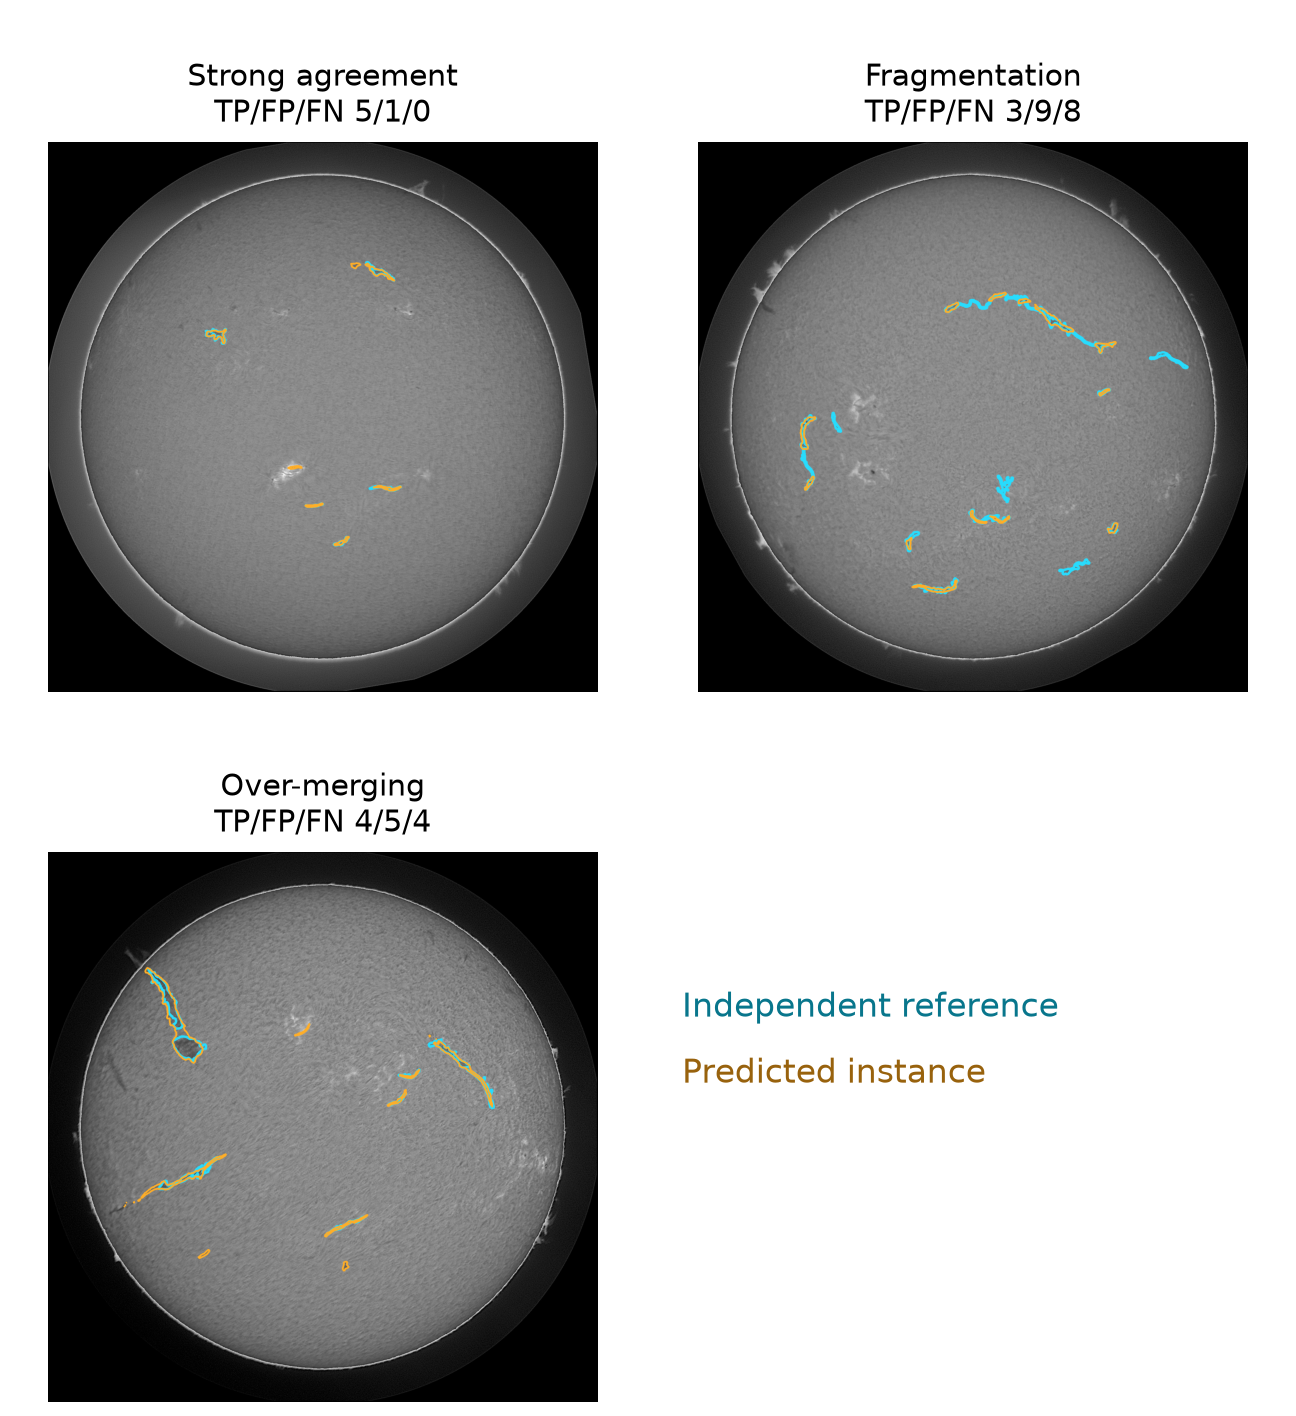
\includegraphics[width=0.99\columnwidth]{examples.png}
\captionof{figure}{Saved OPT-031 predictions on three development images. Cyan outlines show one independent reference and amber outlines show predicted instances. The examples illustrate agreement, fragmentation and over-merging. TP/FP/FN are reference-specific strict matches.}
\label{fig:examples}
\end{minipage}\par\medskip

\clearpage
\section{Evaluation}\label{sec:evaluation}
\subsection{Protocol}
We report the organizers' self-evaluation notebook PQ and also provide strict one-to-one micro-PQ for the final development configuration. For strict matching, prediction and reference instances are paired one-to-one above IoU 0.50. The numerator sums matched IoUs and the denominator is $\mathrm{TP} + 0.5(\mathrm{FP}+\mathrm{FN})$. Aggregation is over independent references. We additionally report semantic union Dice and IoU by reference as measures of pixel overlap. Those semantic measures can remain high when a prediction fragments or merges instances, so we also record both structural error counts.

\subsection{Training ablation}
Table~\ref{tab:ablation} shows each arm's best checkpoint under the common single-view development protocol. F gains 0.00436 notebook PQ over A and reduces the FP count by 44 while keeping the same FN count. C and D individually score below A. E slightly exceeds A and is the best of the three loss candidates C--E. F combines the two loss terms and staged augmentation. The observed gain therefore pertains to the combined recipe on this split. The individual-arm results show no consistent gain from either extra loss alone.

\begin{table}[h]
\caption{Training ablation on 148 development photos. All rows use single-view inference at confidence 0.90 and pixel cutoff 0.50.}
\label{tab:ablation}
\centering
\small
\begin{tabular}{clrr}
\toprule
Arm & Training configuration & Epoch & PQ \\
\midrule
A & Native baseline & 70 & 0.440664 \\
B & Staged augmentation & 70 & 0.440824 \\
C & Boundary loss & 70 & 0.438989 \\
D & Soft-clDice & 60 & 0.438920 \\
E & Boundary and soft-clDice & 80 & 0.440860 \\
F & E with staged augmentation & 80 & \textbf{0.445020} \\
\bottomrule
\end{tabular}
\end{table}

\newpage
\subsection{Inference selection}
With the F checkpoint, three-view inference at 0.90/0.50 raises development notebook PQ by 0.01052 to 0.45554. A subsequent photo-grouped five-fold threshold calibration selected 0.90/0.40 in all five folds. The pooled development notebook PQ is 0.45930, and the strict micro-PQ is 0.45910. Relative to 0.90/0.50, the notebook counts show 79 fewer false positives and 21 more false negatives. Fragmentation decreases from 63 to 52 and merges from 56 to 54. The 5,000-draw photo-clustered bootstrap gives a mean PQ gain of 0.00372 and a 95\% percentile interval of $[0.00038, 0.00711]$. This interval describes threshold variation on the development set with an already selected model and TTA method.

\begin{table}[h]
\caption{F checkpoint inference results. Scores use the notebook evaluator.}
\label{tab:inference}
\centering
\small
\begin{tabular}{llrrr}
\toprule
Split & Method & PQ & FP & FN \\
\midrule
Dev & Identity 0.90/0.50 & 0.44502 & 772 & 845 \\
Dev & 3 views 0.90/0.50 & 0.45554 & 741 & 814 \\
Dev & 3 views 0.90/0.40 & 0.45930 & 662 & 835 \\
Holdout & 3 views 0.90/0.50 & 0.44601 & 777 & 937 \\
\bottomrule
\end{tabular}
\end{table}

\par\medskip\noindent\begin{minipage}{\columnwidth}
\centering
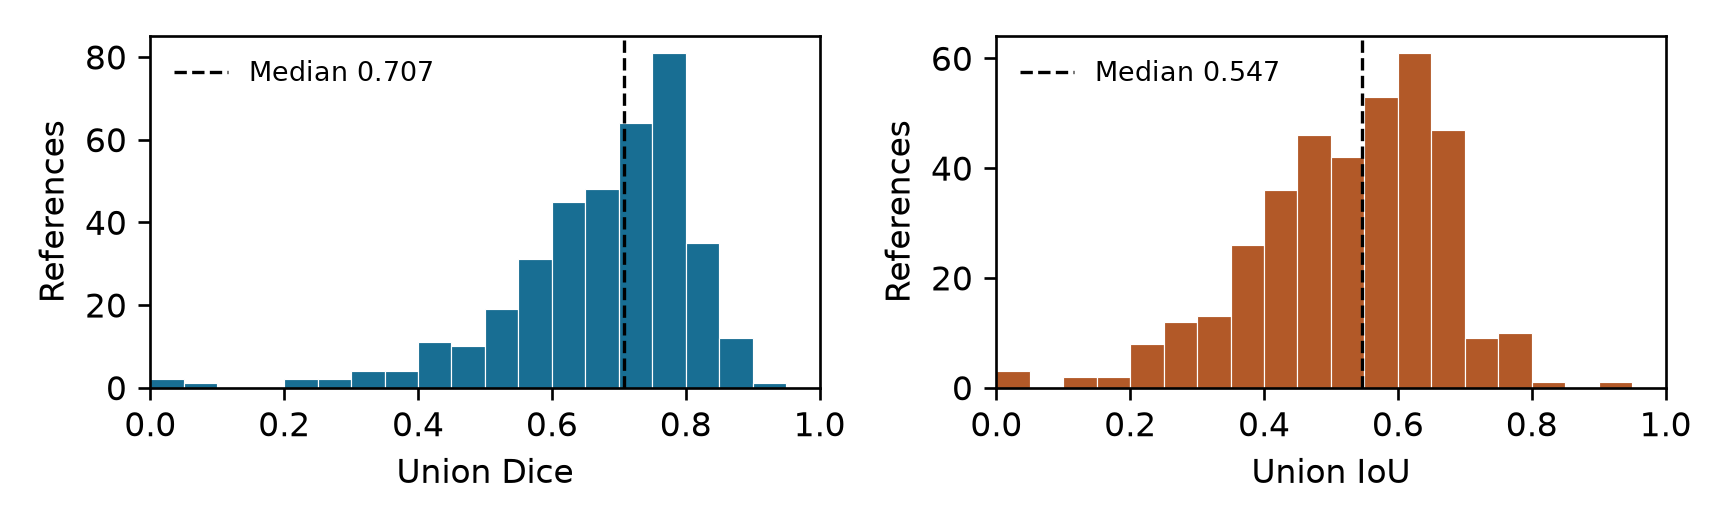
\includegraphics[width=.99\columnwidth]{overlap-distributions.png}
\captionof{figure}{Reference-level union Dice and IoU distributions for the submitted inference configuration on 148 development photos with 372 independent references. Dashed lines indicate medians.}
\label{fig:overlap}
\end{minipage}\par\medskip

\clearpage
\subsection{Holdout and competition results}
The internal holdout contains 148 images with 371 independent references. The earlier three-view 0.90/0.50 configuration achieved PQ 0.44601 there, with 1,630 TP, 777 FP and 937 FN. The holdout was evaluated once after the earlier inference choice. We report that score with its original cutoff. The 0.90/0.40 configuration was selected using development data and has no corresponding holdout run in the archived experiment.

The final competition CSV is Kaggle submission 57372264. Kaggle reported a displayed public score of 0.39. The test labels were unavailable to this pipeline and were excluded from training and selection. The local development PQ and the public score summarize different data.

\subsection{Observed failure cases and limitations}
The saved masks show that the three-view method can separate multiple narrow filaments in the same frame, yet still splits elongated structures and sometimes joins neighboring structures (Figure~\ref{fig:examples}). In the illustrative fragmentation case, three fragmentation events were recorded against the selected reference, with nine false positives and eight false negatives. The over-merging example has two recorded merge events. These counts describe the relation to the displayed reference. Independent annotators may draw different extents or instance boundaries on the same frame.

Our ablation uses one split and seed. Checkpoint selection and inference calibration both use the development split. The threshold cross-fit quantifies sensitivity of a frozen model on that split, while the original holdout result applies to the 0.90/0.50 setting. These limits matter for interpreting small differences between the training arms and the closely spaced threshold candidates. On a future independent photo set, a useful comparison would assess long-structure recall and cross-reference agreement alongside PQ.

\subsection{Reproducibility}
The artifact identifiers bind the report to the selected epoch and archived predictions. The original F checkpoint SHA-256 begins with \texttt{0f6d4bb62ecf}, and the submitted CSV SHA-256 begins with \texttt{67de28e92ba4}. The accompanying manifest gives the full digests, training run ID, inference parameters, and Kaggle submission ID. The inference entry point accepts the official test image directory and loads the frozen F weights directly. The validation script checks the complete input inventory, CSV structure, RLE round-trip and predicted overlap. It compares the generated CSV against the archived submitted CSV by SHA-256.

\newpage
\section{Acknowledgment}\label{sec:acknowledgment}
The organization of the Filament Segmentation Challenge 2026 is partially supported by the U.S. National Science Foundation (NSF) under Grant No. 2209912 and 2433781, directorate for Computer and Information Science and Engineering (CSE), and Office of Advanced Cyberinfrastructure (OAC), and Grant No. 2511630, AST Division Of Astronomical Sciences and MPS Directorate for Mathematical and Physical Sciences.

The Filament Segmentation Challenge 2026 is sponsored by the U.S. National Science Foundation (NSF) National Solar Observatory (NSO).

This work utilizes GONG data obtained by the NSO Integrated Synoptic Program, managed by the National Solar Observatory, which is operated by the Association of Universities for Research in Astronomy (AURA), Inc. under a cooperative agreement with the National Science Foundation and with contribution from the National Oceanic and Atmospheric Administration. The GONG network of instruments is hosted by the Big Bear Solar Observatory, High Altitude Observatory, Learmonth Solar Observatory, Udaipur Solar Observatory, Instituto de Astrofísica de Canarias, and Cerro Tololo Interamerican Observatory.

\bibliographystyle{ACM-Reference-Format}
\bibliography{main}
\end{document}
